% =====================================================================
%  Minicurso: métodos numéricos para leis de conservação --- Encontro 2
%  Compilar com lualatex (fontspec). Tema: beamerthemeatomic.sty
%  Figuras: scripts/make_figs.sh (Python 3 + numpy + matplotlib)
% =====================================================================
\documentclass[aspectratio=169,10pt]{beamer}
\usetheme{atomic}

\usepackage{fontspec}
\IfFontExistsTF{Fira Sans}{\setsansfont{Fira Sans}[Scale=0.94]}{\setsansfont{Latin Modern Sans}}
\usepackage[brazil]{babel}
\usepackage{amsmath,amssymb,mathtools}
\usepackage{booktabs,array}
\usepackage{adjustbox}
\usetikzlibrary{decorations.pathreplacing,shapes.misc,patterns}

\AtBeginDocument{\setlength{\abovedisplayskip}{4pt}\setlength{\belowdisplayskip}{4pt}\setlength{\abovedisplayshortskip}{2pt}\setlength{\belowdisplayshortskip}{2pt}}
\newcommand{\pd}[2]{\dfrac{\partial #1}{\partial #2}}
\newcommand{\dd}{\mathrm{d}}
\newcommand{\Fh}{\widehat F}
\newcommand{\ub}{\bar u}
\newcommand{\jump}[1]{[\![#1]\!]}
\newcommand{\Ah}{\widehat A}
\newcommand{\RP}{u^{\mathrm{RP}}}
\newcommand{\lh}{\hat\lambda}
\newcommand{\ah}{\hat\alpha}
\newcommand{\rh}{\hat r}

\title[Minicurso: leis de conservação]{Volumes finitos: upwind, Godunov\\ e solvers de Riemann aproximados}
\subtitle{Minicurso de métodos numéricos para leis de conservação --- Encontro 2 de 4}
\author{Prof. Dr. Ulisses A. Maciel Neto}
\institute{Projeto ATOMIC --- Meta 2 (CTMSP / Ibmec-SP)}
\date{Outubro de 2026}

\begin{document}

\begin{frame}[plain,noframenumbering]
\titlepage
\end{frame}

\begin{frame}{Os quatro encontros}
\begin{center}
\begin{tikzpicture}[x=1cm,y=1cm,
  enc/.style={draw=atomicazul,fill=atomicfundo,rounded corners=3pt,text width=2.95cm,align=center,minimum height=2.1cm,font=\small},
  feito/.style={enc,draw=atomiccinza,text=black!55},
  hoje/.style={enc,fill=atomiclaranja!15,draw=atomiclaranja,line width=1pt}]
\node[feito] (e1) at (0,0) {\textbf{1. Leis de conservação}\\[2pt]\footnotesize hiperbolicidade, choques, soluções fracas, entropia, estabilidade};
\node[hoje] (e2) at (3.45,0) {\textbf{2. Volumes finitos}\\[2pt]\footnotesize problema de Riemann, Godunov, fluxos numéricos};
\node[enc] (e3) at (6.9,0) {\textbf{3. Ordem alta}\\[2pt]\footnotesize reconstrução, limitadores, rDG($P_0P_1$), positividade};
\node[enc] (e4) at (10.35,0) {\textbf{4. Escoamento bifásico}\\[2pt]\footnotesize sete equações, fase evanescente, esquema corrigido};
\foreach \a/\b in {e1/e2,e2/e3,e3/e4}{\draw[-{Stealth[length=6pt]},atomicazul,thick] (\a) -- (\b);}
\node[below=0.25cm of e1,font=\footnotesize,text=black!55] {feito};
\node[below=0.25cm of e2,font=\footnotesize,text=atomiclaranja] {hoje};
\end{tikzpicture}
\end{center}
\vspace{0.2cm}
\begin{itemize}
\item No Encontro 1 vimos \emph{o que} se quer aproximar: o balanço integral, as ondas, os choques e a entropia. Hoje construímos \emph{a ferramenta}: o fluxo numérico na face.
\item Tudo o que vem depois (ordem alta, bifásico) usa o fluxo de hoje como peça básica: o Encontro 3 muda o que se entrega ao fluxo, não o fluxo.
\end{itemize}
\end{frame}

\begin{frame}{Roteiro de hoje}
\begin{columns}[T]
\begin{column}{0.5\textwidth}
\begin{enumerate}
\item Volumes finitos e upwind: o esquema, o fluxo numérico e a sua dissipação
\item O problema de Riemann: Burgers (choque, rarefação, caso sônico) e Euler
\item O método de Godunov: reconstruir, evoluir, fazer a média
\end{enumerate}
\end{column}
\begin{column}{0.5\textwidth}
\begin{enumerate}\setcounter{enumi}{3}
\item O solver de Roe: linearizar na face; correção de entropia; positividade; outros fluxos em uma linha
\item Síntese e exercício para o próximo encontro
\end{enumerate}
\end{column}
\end{columns}
\vspace{0.3cm}
\begin{mensagem}
Fio condutor: a física entra num único lugar, o fluxo na face. Dados $u_L$ e $u_R$, qual é $\Fh(u_L,u_R)$? Upwind responde no caso linear, Godunov responde sempre, Roe responde quase sempre e mais barato.
\end{mensagem}
\end{frame}


% =====================================================================
\section{Volumes finitos e upwind}

\begin{frame}{O esquema de volumes finitos}
\begin{definicao}{Esquema conservativo de volumes finitos (explícito, três pontos)}
Células $K_j=[x_{j-1/2},x_{j+1/2}]$ de largura $h$, médias $\ub_j^{\,n}\approx\frac1h\int_{K_j}u(x,t^n)\,\dd x$, passo $\Delta t$:
\[
\ub_j^{\,n+1}=\ub_j^{\,n}-\frac{\Delta t}{h}\Big(\Fh_{j+1/2}^{\,n}-\Fh_{j-1/2}^{\,n}\Big),\qquad
\Fh_{j+1/2}^{\,n}=\Fh\big(\ub_j^{\,n},\ub_{j+1}^{\,n}\big),
\]
com \textbf{fluxo numérico} $\Fh(u_L,u_R)$ consistente, $\Fh(u,u)=f(u)$, e contínuo nos dois argumentos.
\end{definicao}
\begin{columns}[T]
\begin{column}{0.5\textwidth}
\begin{itemize}
\item É a forma integral do Encontro 1 com uma única aproximação: o fluxo médio na face durante o passo, trocado por uma função dos dois estados vizinhos.
\item Somando em $j$, os fluxos interiores cancelam: conservação discreta exata, logo choques na velocidade certa (Lax--Wendroff, Encontro 1).
\end{itemize}
\end{column}
\begin{column}{0.5\textwidth}
\begin{itemize}
\item Contornos por \textbf{células fantasma}: transmissivo copia a vizinha, periódico envolve, parede reflete a velocidade. Passo: $\Delta t=\mathrm{CFL}\cdot h/\max_j|\lambda|_{\max}$, com $\mathrm{CFL}\le1$.
\end{itemize}
\begin{intuicao}
Dois esquemas de volumes finitos só diferem na resposta a uma pergunta: quanto atravessa a face quando os dois lados discordam? Esquema \emph{é} fluxo numérico.
\end{intuicao}
\end{column}
\end{columns}
\end{frame}

\begin{frame}{Todo fluxo numérico é ``média central mais dissipação''}
\begin{teorema}{Forma viscosa de um fluxo numérico}
\[
\Fh(u_L,u_R)=\underbrace{\tfrac12\big[f(u_L)+f(u_R)\big]}_{\text{média central}}\;-\;\underbrace{\tfrac12\,Q\,(u_R-u_L)}_{\text{dissipação numérica}},
\qquad Q=\text{coeficiente de viscosidade numérica.}
\]
\end{teorema}
\begin{columns}[T]
\begin{column}{0.46\textwidth}
\begin{center}\scriptsize
\begin{tabular}{@{}ll@{}}
\toprule
fluxo & $Q$ (advecção, $f=au$)\\
\midrule
central & $0$: instável (explícito)\\
Lax--Wendroff & $\nu|a|$: ordem 2, oscila\\
upwind & $|a|$: o menor $Q$ sem oscilações\\
Lax--Friedrichs & $h/\Delta t$: o maior $Q$ estável\\
Rusanov & $\max\{|f'(u_L)|,|f'(u_R)|\}$\\
Godunov, Roe & o que as ondas pedem (Partes 3 e 4)\\
\bottomrule
\end{tabular}
\end{center}
\end{column}
\begin{column}{0.54\textwidth}
\begin{itemize}
\item Na advecção, $Q$ \emph{é} a viscosidade da equação modificada (Encontro 1): estável sse $\nu|a|\le Q\le h/\Delta t$, sem extremos novos sse $|a|\le Q\le h/\Delta t$.
\item Esquemas que não criam extremos (\emph{monótonos}) são TVD e convergem para a solução de entropia (Harten, Hyman e Lax, 1976; Crandall e Majda, 1980): é a teoria que fica nos bastidores de tudo o que segue.
\end{itemize}
\end{column}
\end{columns}
\begin{mensagem}
Escolher o fluxo é escolher quanta viscosidade pôr em cada face: pouca oscila ou explode, muita borra. A física das ondas diz o mínimo necessário.
\end{mensagem}
\end{frame}

\begin{frame}{O ``botão'' da dissipação: de Lax--Wendroff a Lax--Friedrichs}
\begin{center}
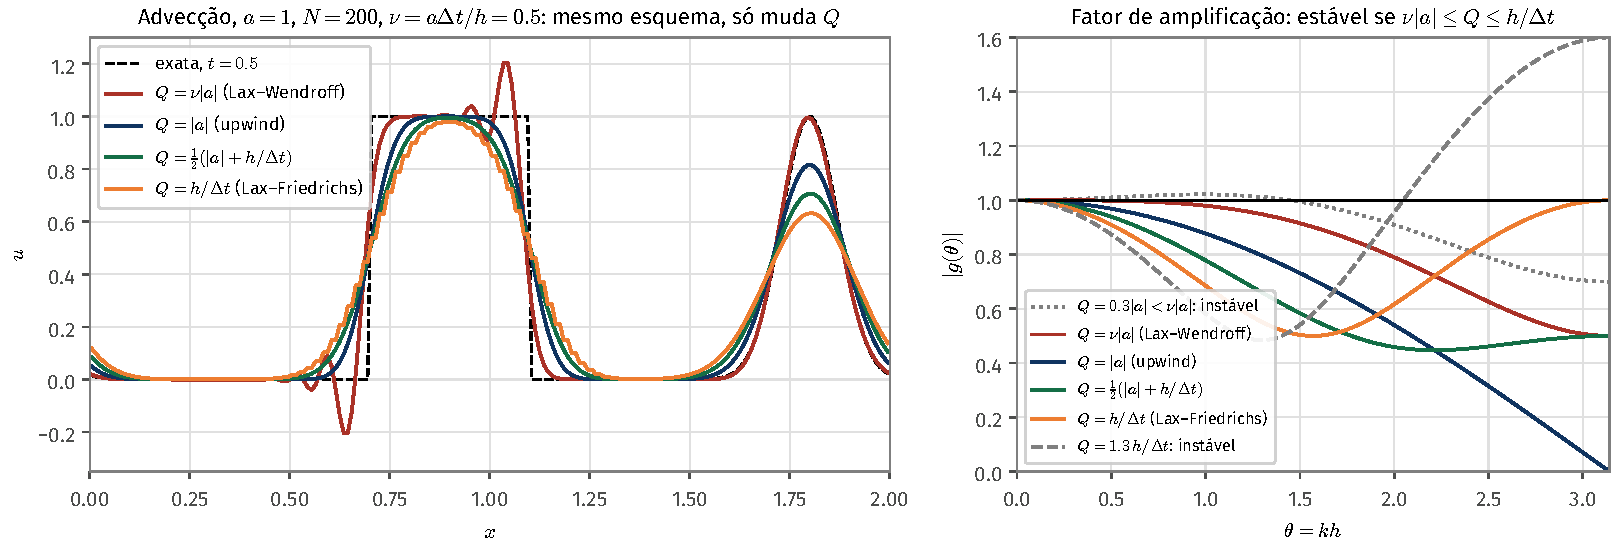
\includegraphics[width=\textwidth,height=0.66\textheight,keepaspectratio]{figs/fluxo_dissipacao.pdf}
\end{center}
\vspace{-0.15cm}
{\footnotesize Mesmo dado, mesmo esquema, só muda $Q$ ($\nu=0.5$). À esquerda: $Q=\nu|a|$ oscila; $Q=|a|$ é o mais nítido que não oscila; $Q=h/\Delta t$ é o mais borrado. À direita, $|g(\theta)|$: abaixo de $\nu|a|$ ou acima de $h/\Delta t$ há modos com $|g|>1$ e o esquema explode.}
\end{frame}

\begin{frame}{Upwind como fluxo numérico: cada onda tem o seu lado}
\begin{columns}[T]
\begin{column}{0.54\textwidth}
\begin{definicao}{Fluxo upwind}
Advecção, $f=au$: $\Fh=a^+u_L+a^-u_R$, com $a^\pm=\tfrac12(a\pm|a|)$; isto é, $Q=|a|$. Sistema linear $u_t+Au_x=0$, $A=R\Lambda R^{-1}$, $|A|=R|\Lambda|R^{-1}$:
\[
\Fh=A^+u_L+A^-u_R=\tfrac12A\,(u_L+u_R)-\tfrac12|A|\,(u_R-u_L).
\]
\end{definicao}
\begin{itemize}
\item Decompondo o salto em ondas, $u_R-u_L=\sum_p\alpha_p r_p$ ($\alpha=R^{-1}\Delta u$), o fluxo é $f(u_L)$ mais as ondas que vão para a esquerda: $\Fh=f(u_L)+\sum_{\lambda_p<0}\lambda_p\alpha_pr_p$.
\item É a solução \emph{exata} do problema de Riemann linear lida na face: upwind é Godunov no caso linear.
\item Escalar não linear com $f'$ de sinal fixo: $f(u_L)$ ou $f(u_R)$. Se $f'$ troca de sinal entre $u_L$ e $u_R$ (Burgers, $u_L<0<u_R$), nenhum dos dois serve: é o \textbf{ponto sônico}, Parte 2.
\end{itemize}
\end{column}
\begin{column}{0.46\textwidth}
\begin{center}
\begin{tikzpicture}[x=1cm,y=0.8cm,font=\scriptsize]
\draw[-{Stealth}] (-2.6,0)--(2.8,0) node[right]{$x$}; \draw[-{Stealth},atomiclaranja,dashed,thick] (0,0)--(0,1.9) node[above,text=atomiclaranja]{face};
\draw[atomicazul,thick] (0,0)--(-1.7,1.7) node[above,text=atomicazul]{$\lambda_1<0$};
\draw[atomicazul,thick] (0,0)--(0.8,1.7) node[above,text=atomicazul]{$\lambda_2$};
\draw[atomicazul,thick] (0,0)--(2.0,1.7) node[above,text=atomicazul]{$\lambda_3$};
\node at (-2.0,0.4) {$u_L$}; \node at (2.3,0.4) {$u_R$};
\node[align=center] at (-0.5,1.3) {$u_1^*=u_L+\alpha_1 r_1$};
\node[align=center] at (1.3,0.7) {$u_2^*=u_1^*+\alpha_2 r_2$};
\end{tikzpicture}
\end{center}
\begin{intuicao}
$|A|$ dissipa cada onda com a sua própria $|\lambda_p|$: nem mais, nem menos. Rusanov usa $\max_p|\lambda_p|$ em todas e borra as ondas lentas (o contato em Euler, as ondas de $\alpha$ no bifásico). Upwind é olhar para a célula de onde cada onda vem.
\end{intuicao}
\end{column}
\end{columns}
\end{frame}


% =====================================================================
\section{O problema de Riemann}

\begin{frame}{Burgers: choque ou rarefação, e o caso sônico}
\begin{teorema}{Solução do problema de Riemann para $f$ convexa}
\begin{itemize}
\item $u_L>u_R$: \textbf{choque}, $u=u_L$ se $x<st$ e $u_R$ se $x>st$, com $s=\frac{f(u_R)-f(u_L)}{u_R-u_L}$ (Burgers: $s=\frac{u_L+u_R}{2}$).
\item $u_L<u_R$: \textbf{rarefação}, $u=u_L$ se $x<f'(u_L)\,t$, $u_R$ se $x>f'(u_R)\,t$ e $f'(u)=x/t$ no leque (Burgers: $u=x/t$).
\end{itemize}
\end{teorema}
\begin{columns}[T]
\begin{column}{0.5\textwidth}
\begin{definicao}{Fluxo de Godunov para Burgers}
O valor na face é $\RP(0)$, a solução em $x/t=0$:
\[
\Fh^{\mathrm G}(u_L,u_R)=\max\big\{f(u_L^+),\,f(u_R^-)\big\},
\]
com $u^+=\max(u,0)$ e $u^-=\min(u,0)$. (Caso convexo geral: $\min_{[u_L,u_R]}f$ se $u_L\le u_R$, $\max_{[u_R,u_L]}f$ se $u_L>u_R$.)
\end{definicao}
\end{column}
\begin{column}{0.5\textwidth}
\begin{center}\scriptsize
\begin{tabular}{@{}lll@{}}
\toprule
situação (Burgers) & estado na face & fluxo\\
\midrule
$u_L>u_R$, $s>0$ & $u_L$ & $f(u_L)$\\
$u_L>u_R$, $s<0$ & $u_R$ & $f(u_R)$\\
$0\le u_L<u_R$ & $u_L$ & $f(u_L)$\\
$u_L<u_R\le0$ & $u_R$ & $f(u_R)$\\
$u_L<0<u_R$ (sônico) & $0$ & $f(0)=0$\\
\bottomrule
\end{tabular}
\end{center}
\begin{intuicao}
No caso sônico a face está \emph{dentro} do leque, onde a característica está parada: o valor lido não é $u_L$ nem $u_R$. É aqui que o upwind ingênuo e o Roe sem correção erram.
\end{intuicao}
\end{column}
\end{columns}
\end{frame}

\begin{frame}{Os três problemas de Riemann de Burgers}
\begin{center}
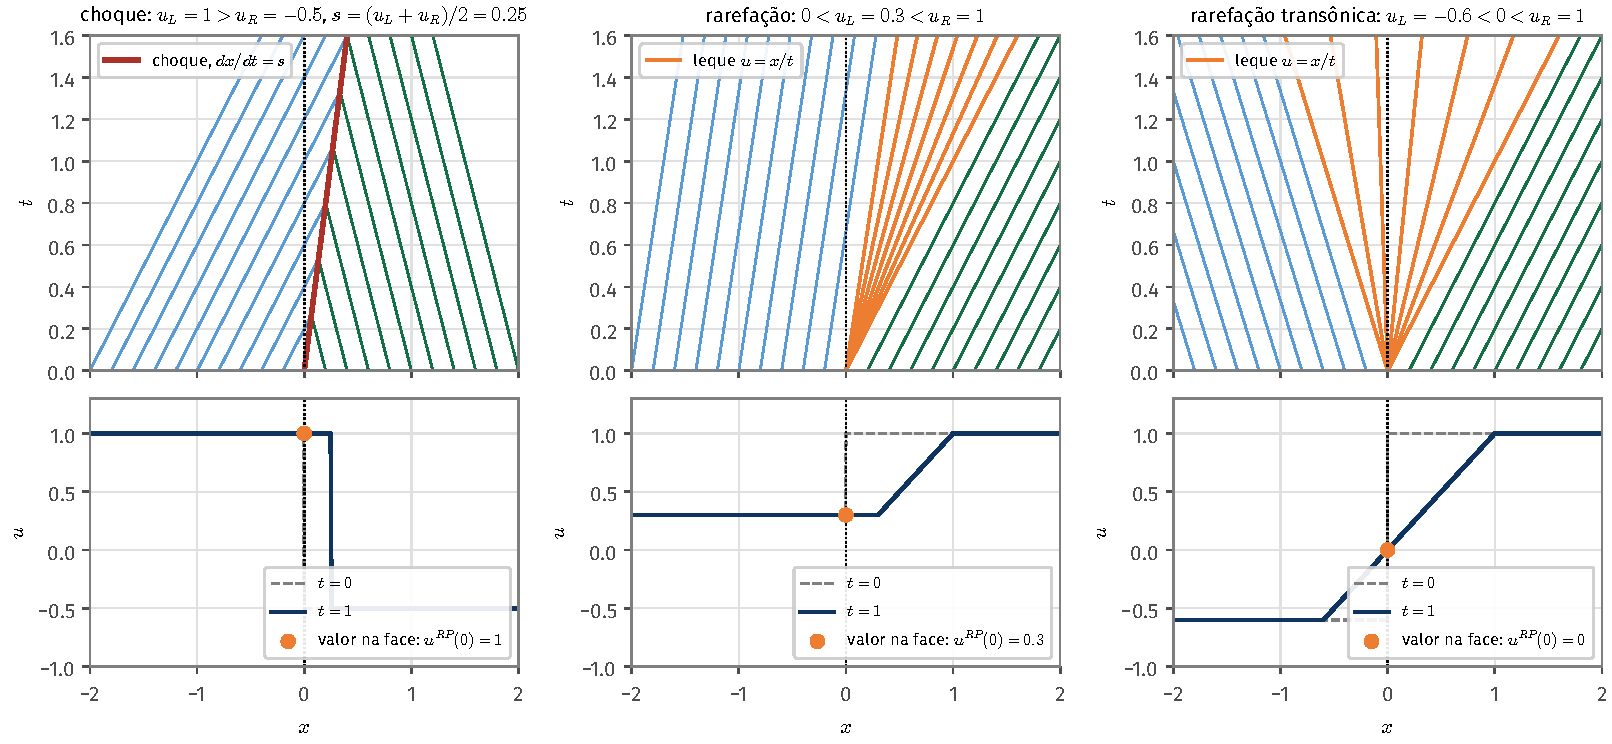
\includegraphics[width=\textwidth,height=0.7\textheight,keepaspectratio]{figs/riemann_burgers.pdf}
\end{center}
\vspace{-0.2cm}
{\footnotesize Em cima, características e onda no plano $x$--$t$; embaixo, a solução em $t=1$ e o valor lido na face $x=0$ (ponto laranja), que define o fluxo de Godunov $f(\RP(0))$. No caso transônico as características divergem da face e o valor lido é o ponto sônico, $u=0$.}
\end{frame}

\begin{frame}{Euler: a solução exata cabe numa equação escalar}
\begin{columns}[T]
\begin{column}{0.58\textwidth}
\begin{itemize}
\item Três ondas: a 1-onda ($u-c$) e a 3-onda ($u+c$), choque ou rarefação cada, e o contato no meio. Na região \emph{estrela}, $p^*$ e $u^*$ são os mesmos dos dois lados; $\rho^*_L\neq\rho^*_R$.
\item Cada onda externa liga $u^*$ a $p^*$: $u^*=u_L-f_L(p^*)=u_R+f_R(p^*)$, com $f_K$ dada por Rankine--Hugoniot (se choque) ou pelo invariante de Riemann (se rarefação). Igualando:
\[
f(p^*)\equiv f_L(p^*)+f_R(p^*)+(u_R-u_L)=0 .
\]
\item $f$ é crescente e côncava: Newton converge em 3--5 iterações. Depois $u^*$ sai de $f_L$, $f_R$, e a solução é amostrada em $x/t$. Fórmulas em Toro (cap.\ 4) e no script \texttt{riemann\_exato.py} fornecido.
\item Sod (Encontro 1): $p^*=0.303$, $u^*=0.927$; é assim que a ``exata'' das figuras é calculada.
\end{itemize}
\end{column}
\begin{column}{0.42\textwidth}
\begin{center}
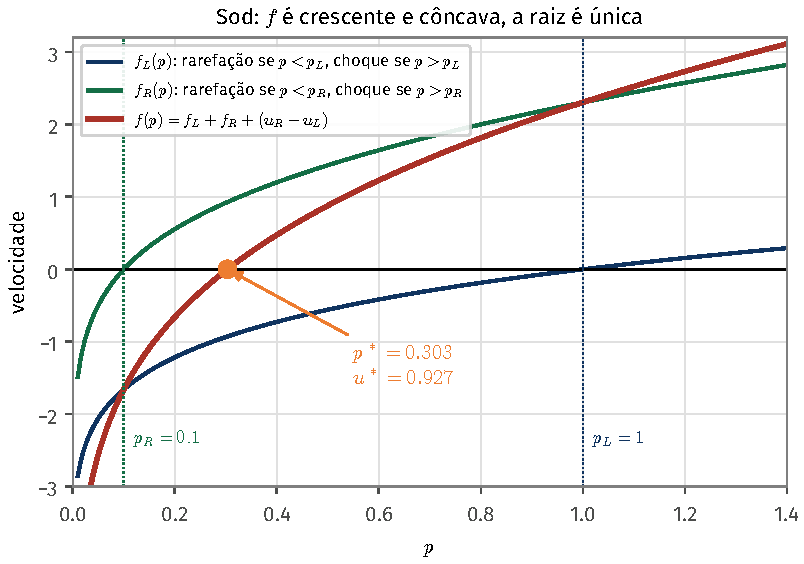
\includegraphics[width=0.95\textwidth]{figs/euler_pfunc.pdf}
\end{center}
\begin{mensagem}
O esquema usa da solução exata um único valor, em $x/t=0$; o custo é um Newton por face e por passo.
\end{mensagem}
\end{column}
\end{columns}
\end{frame}


% =====================================================================
\section{O método de Godunov}

\begin{frame}{Godunov (1959): reconstruir, evoluir, fazer a média}
\begin{center}
\begin{tikzpicture}[x=1cm,y=1cm,font=\scriptsize]
\begin{scope}
\draw[gray!60] (0,0)--(4,0);
\draw[gray!70,dashed,thick] plot[smooth] coordinates {(0,0.5)(0.7,0.65)(1.4,1.0)(2.1,1.35)(2.8,1.45)(3.5,1.3)(4,1.15)};
\foreach \x in {0,1,2,3,4}{\draw[black!35,dashed] (\x,0)--(\x,1.7);}
\draw[atomicazul,line width=1.5pt] (0,0.6)--(1,0.6) (1,1.05)--(2,1.05) (2,1.42)--(3,1.42) (3,1.28)--(4,1.28);
\node[anchor=north] at (2,-0.1) {(a) reconstruir: $\tilde u^n(x)=\ub_j^{\,n}$ em $K_j$};
\end{scope}
\begin{scope}[shift={(5.2,0)}]
\draw[gray!60] (0,0)--(4,0); \draw[gray!60] (0,1.5)--(4,1.5);
\foreach \x in {0,1,2,3,4}{\draw[black!35,dashed] (\x,0)--(\x,1.5);}
\foreach \x in {1,2,3}{\fill[atomiclaranja!25] (\x,0)--({\x-0.45},1.5)--({\x+0.45},1.5)--cycle;
  \draw[atomicvermelho,thick] (\x,0)--({\x+0.45},1.5); \draw[atomicazul,thick] (\x,0)--({\x-0.45},1.5); \draw[atomiclaranja,thick,dashed] (\x,0)--({\x+0.15},1.5);}
\node[left] at (0,0) {$t^n$}; \node[left] at (0,1.5) {$t^{n+1}$};
\node[anchor=north,align=center] at (2,-0.1) {(b) evoluir: um problema de Riemann por face;\\ as ondas não chegam às faces vizinhas (CFL $\le1$)};
\end{scope}
\begin{scope}[shift={(10.4,0)}]
\draw[gray!60] (0,0)--(4,0);
\foreach \x in {0,1,2,3,4}{\draw[black!35,dashed] (\x,0)--(\x,1.7);}
\draw[atomicazul!40,line width=1pt] (0,0.6)--(1,0.6) (1,1.05)--(2,1.05) (2,1.42)--(3,1.42) (3,1.28)--(4,1.28);
\draw[atomiclaranja,line width=1.5pt] (0,0.62)--(1,0.62) (1,0.98)--(2,0.98) (2,1.33)--(3,1.33) (3,1.33)--(4,1.33);
\node[anchor=north] at (2,-0.1) {(c) média: $\ub_j^{\,n+1}=\frac1h\int_{K_j}\tilde u(x,t^{n+1})\,\dd x$};
\end{scope}
\end{tikzpicture}
\end{center}
\vspace{0.1cm}
\begin{columns}[T]
\begin{column}{0.5\textwidth}
\begin{enumerate}
\item \textbf{Reconstruir}: das médias $\ub_j^{\,n}$, a função constante por célula.
\item \textbf{Evoluir}: resolver \emph{exatamente} a lei de conservação com esse dado durante $\Delta t$: uma sequência de problemas de Riemann, um por face.
\item \textbf{Média}: projetar $\tilde u(\cdot,t^{n+1})$ de volta em constantes por célula.
\end{enumerate}
\end{column}
\begin{column}{0.5\textwidth}
\begin{intuicao}
O único erro do método está na média: a evolução é exata. Projetar perde informação, e é isso que aparece como difusão numérica. Ordem alta (Encontro 3) é \emph{reconstruir melhor} antes de evoluir.
\end{intuicao}
\end{column}
\end{columns}
\end{frame}

\begin{frame}{O método de Godunov: definição e propriedades}
\begin{definicao}{Fluxo de Godunov}
Seja $\RP(x/t;u_L,u_R)$ a solução de entropia do problema de Riemann com estados $u_L$ e $u_R$:
\[
\Fh^{\mathrm G}(u_L,u_R)=f\big(\RP(0;u_L,u_R)\big).
\]
Como a solução de Riemann depende só de $x/t$, na face ela vale $\RP(0)$ durante todo o passo: o fluxo médio sai \emph{exato} enquanto as ondas das faces vizinhas não chegam (CFL $\le1$).
\end{definicao}
\begin{columns}[T]
\begin{column}{0.5\textwidth}
\begin{itemize}
\item Advecção: upwind. Sistema linear: upwind por onda. Burgers: a fórmula do $\max/\min$. Euler: o solver exato da Parte 2.
\item Não cria extremos novos, respeita a entropia (abre a rarefação certa, Encontro 1) e, em sistemas, é o padrão-ouro de primeira ordem.
\end{itemize}
\end{column}
\begin{column}{0.5\textwidth}
\begin{itemize}
\item Primeira ordem: borra contatos como todo esquema de ordem 1. Godunov (1959) provou também que \emph{qualquer} esquema linear sem extremos novos é no máximo de ordem 1: daí os limitadores do Encontro 3.
\item Custo: um problema de Riemann exato por face e por passo (Newton, em Euler).
\end{itemize}
\end{column}
\end{columns}
\begin{mensagem}
Godunov responde à pergunta da face do único modo fiel: deixa a física decidir. Roe tenta dar a mesma resposta mais barato.
\end{mensagem}
\end{frame}

\begin{frame}{Godunov no tubo de Sod: o que a primeira ordem faz com cada onda}
\begin{center}
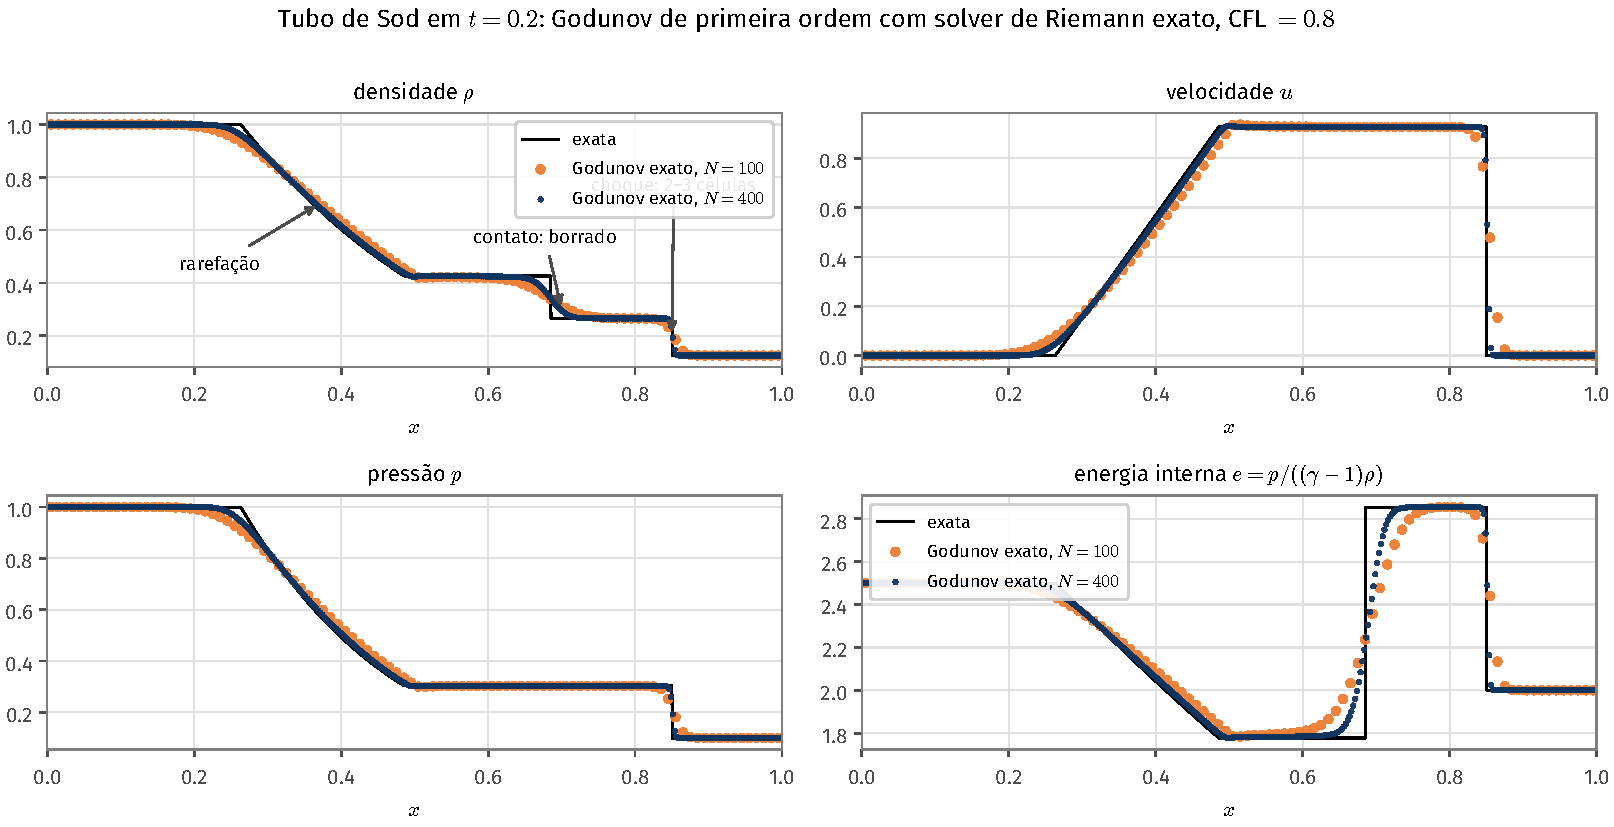
\includegraphics[width=\textwidth,height=0.6\textheight,keepaspectratio]{figs/godunov_sod.pdf}
\end{center}
\vspace{-0.2cm}
{\footnotesize Choque: 2--3 células e não piora com o tempo (as características convergem para ele e o recomprimem). Contato: borrado e cada vez mais largo, porque nada o comprime: é um salto apenas transportado, como o degrau da advecção. Rarefação: boa. Dobrar $N$ reduz o erro, mas menos que pela metade.}
\end{frame}


% =====================================================================
\section{O solver de Roe}

\begin{frame}{Por que aproximar, e a ideia de Roe (1981)}
\begin{columns}[T]
\begin{column}{0.5\textwidth}
\begin{itemize}
\item O exato custa um Newton por face e passo; com gás real (IAPWS) nem há forma fechada, e nas sete equações a solução exata nem é conhecida.
\item O esquema só usa $\RP(0)$, e a média apaga o resto: basta um fluxo ``certo o bastante''.
\item Ideia: trocar $f'(u)$ por uma matriz \emph{constante} $\Ah(u_L,u_R)$ na face e resolver o problema de Riemann \emph{linear} exatamente (Parte 1).
\end{itemize}
\begin{intuicao}
Roe pergunta: ``qual matriz constante faria $(u_L,u_R)$ obedecer a Rankine--Hugoniot?'' Com ela, a face vê um problema linear que já carrega a velocidade certa do choque.
\end{intuicao}
\end{column}
\begin{column}{0.5\textwidth}
\begin{definicao}{Matriz de Roe}
$\Ah(u_L,u_R)$ é uma matriz de Roe para o fluxo $f$ se
\begin{enumerate}
\item[(i)] $\Ah\,(u_R-u_L)=f(u_R)-f(u_L)$ (Rankine--Hugoniot exata);
\item[(ii)] tem autovalores reais e autovetores independentes;
\item[(iii)] $\Ah(u,u)=f'(u)$ (consistência).
\end{enumerate}
\end{definicao}
\begin{itemize}
\item Consequência de (i): num choque ou contato isolado de velocidade $s$, $\Ah\Delta u=s\Delta u$, e o problema linear reproduz a descontinuidade \emph{exatamente}, à velocidade certa.
\item Burgers: $\hat a=\frac{u_L+u_R}{2}$, pois $\hat a\,(u_R-u_L)=\frac{u_R^2-u_L^2}{2}$. É a velocidade do choque.
\end{itemize}
\end{column}
\end{columns}
\end{frame}

\begin{frame}{O fluxo de Roe: onde acerta e onde erra}
\begin{definicao}{Fluxo de Roe}
Com $\Ah=\hat R\hat\Lambda\hat R^{-1}$ e intensidades $\ah=\hat R^{-1}(u_R-u_L)$, o upwind por onda do problema linearizado é
\[
\Fh^{\mathrm{Roe}}=\tfrac12\big[f(u_L)+f(u_R)\big]-\tfrac12\sum_{p}|\lh_p|\,\ah_p\,\rh_p
\;=\;f(u_L)+\sum_{\lh_p<0}\lh_p\,\ah_p\,\rh_p ,\qquad\text{isto é, } Q=|\Ah|.
\]
\end{definicao}
\begin{columns}[T]
\begin{column}{0.52\textwidth}
\begin{itemize}
\item Burgers: $\Fh=\frac12[f(u_L)+f(u_R)]-\frac12\big|\frac{u_L+u_R}{2}\big|(u_R-u_L)$.
\item Choque: como $\hat a=s$, dá $f(u_L)$ se $s>0$ e $f(u_R)$ se $s<0$: \textbf{igual ao Godunov}. Rarefação com $f'$ de sinal fixo: também igual.
\item Rarefação transônica ($u_L<0<u_R$): Godunov dá $f(0)=0$; Roe dá $f(u_L)$ ou $f(u_R)$ e, se $u_L=-u_R$, $Q=0$: o salto fica parado. É o choque de expansão do Encontro 1.
\end{itemize}
\end{column}
\begin{column}{0.48\textwidth}
\begin{atencao}{O que a linearização não enxerga}
Ela troca o leque por um único salto. Quando as características \emph{divergem} dos dois lados da face ($\lambda(u_L)<0<\lambda(u_R)$), nenhum salto é a resposta: a face está dentro do leque e precisa de uma dissipação da ordem da abertura dele.
\end{atencao}
\end{column}
\end{columns}
\end{frame}

\begin{frame}{A correção de entropia}
\begin{definicao}{Correção de Harten e Hyman (1983)}
Para a onda $p$, sejam $\lambda_p^L$ e $\lambda_p^R$ as velocidades características reais nos estados à esquerda e à direita da onda (Burgers: $u_L$ e $u_R$). Se $\lambda_p^L<0<\lambda_p^R$ (onda \textbf{transônica}), o salto único de velocidade $\lh_p$ é trocado por dois, de velocidades $\lambda_p^L$ e $\lambda_p^R$, com frações $\beta_p$ e $1-\beta_p$ da intensidade, $\beta_p=\dfrac{\lambda_p^R-\lh_p}{\lambda_p^R-\lambda_p^L}$ (escolhido para conservar). Na fórmula $\Fh=f(u_L)+\sum_p\min(\lh_p,0)\,\ah_p\rh_p$, a onda transônica entra com $\beta_p\lambda_p^L$: só a parte que vai para a esquerda cruza a face.
\end{definicao}
\begin{columns}[T]
\begin{column}{0.5\textwidth}
\begin{itemize}
\item Burgers transônico: $\beta=\tfrac12$ e $\Fh=\tfrac12u_Lu_R\le0$: a face recebe dissipação e o leque se abre (figura a seguir).
\item Fora das ondas transônicas nada muda: choques e contatos continuam exatos.
\end{itemize}
\end{column}
\begin{column}{0.5\textwidth}
\begin{itemize}
\item Versão mais simples (Harten, 1983): $|\lh_p|\to\frac{\lh_p^2+\delta_p^2}{2\delta_p}$ se $|\lh_p|<\delta_p$, com $\delta_p$ a abertura do leque: um mínimo de dissipação onde o autovalor troca de sinal.
\end{itemize}
\begin{mensagem}
A correção devolve ao Roe a informação de que, numa rarefação, o leque tem largura e a face está dentro dele.
\end{mensagem}
\end{column}
\end{columns}
\end{frame}

\begin{frame}{Godunov, Roe e Rusanov em Burgers: onde coincidem e onde não}
\begin{center}
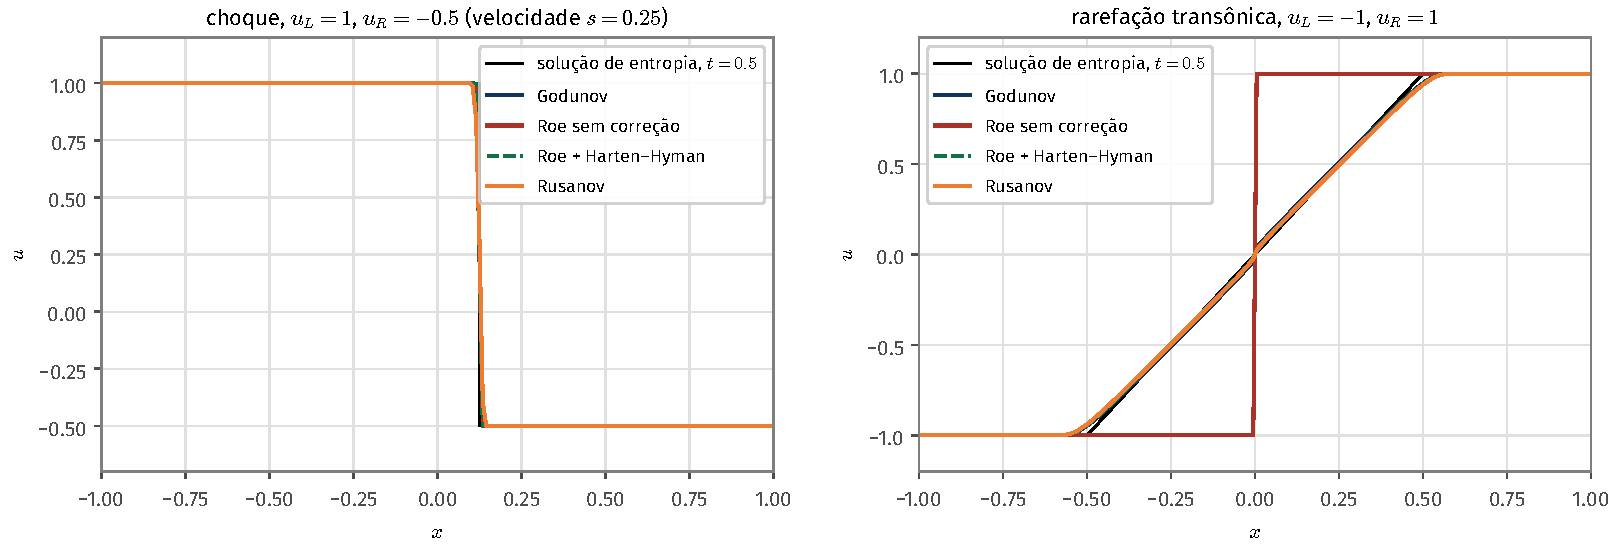
\includegraphics[width=\textwidth,height=0.62\textheight,keepaspectratio]{figs/burgers_godunov_roe.pdf}
\end{center}
\vspace{-0.15cm}
{\footnotesize $N=200$, CFL $=0.8$, $t=0.5$. À esquerda, choque com $s=0.25$: Godunov e Roe (com ou sem correção) coincidem, porque $\hat a=s$; Rusanov, com $Q=\max\{|u_L|,|u_R|\}>|s|$, borra um pouco mais. À direita, rarefação transônica: o Roe sem correção mantém o choque de expansão ($Q=0$ na face sônica); com Harten--Hyman abre o leque como o Godunov.}
\end{frame}

\begin{frame}{Roe para Euler: as médias de Roe}
\begin{definicao}{Médias de Roe (gás ideal), com $H=(E+p)/\rho$ a entalpia total específica}
\[
\hat u=\frac{\sqrt{\rho_L}\,u_L+\sqrt{\rho_R}\,u_R}{\sqrt{\rho_L}+\sqrt{\rho_R}},\qquad
\hat H=\frac{\sqrt{\rho_L}\,H_L+\sqrt{\rho_R}\,H_R}{\sqrt{\rho_L}+\sqrt{\rho_R}},\qquad
\hat c^{\,2}=(\gamma-1)\Big(\hat H-\tfrac12\hat u^2\Big).
\]
$\Ah$ é a jacobiana de Euler avaliada em $(\hat u,\hat H,\hat c)$: $\lh_{1,2,3}=\hat u-\hat c,\ \hat u,\ \hat u+\hat c$;\ \
$\rh_1=(1,\,\hat u-\hat c,\,\hat H-\hat u\hat c)^{\!\top}$, $\rh_2=(1,\,\hat u,\,\tfrac12\hat u^2)^{\!\top}$, $\rh_3=(1,\,\hat u+\hat c,\,\hat H+\hat u\hat c)^{\!\top}$.
\end{definicao}
\begin{columns}[T]
\begin{column}{0.52\textwidth}
\begin{teorema}{Intensidades das ondas, com $\Delta(\cdot)=(\cdot)_R-(\cdot)_L$}
\vspace{-0.3cm}
\[
{\small\begin{aligned}
\ah_2&=\frac{\gamma-1}{\hat c^{\,2}}\Big[\Delta\rho\,(\hat H-\hat u^2)+\hat u\,\Delta(\rho u)-\Delta E\Big],\\
\ah_1&=\frac{1}{2\hat c}\Big[\Delta\rho\,(\hat u+\hat c)-\Delta(\rho u)-\hat c\,\ah_2\Big],\\
\ah_3&=\Delta\rho-\ah_1-\ah_2 .
\end{aligned}}
\]
\end{teorema}
\end{column}
\begin{column}{0.48\textwidth}
\begin{itemize}
\item Por face: médias $\to$ $\lh_p$, $\rh_p$, $\ah_p$ $\to$ correção de entropia nas ondas 1 e 3 $\to$ $\Fh=\frac12(f_L+f_R)-\frac12\sum_p|\lh_p|\ah_p\rh_p$.
\item Os pesos $\sqrt\rho$ são o que faz (i) valer exatamente para o gás ideal. Para gás real e para as sete equações há generalizações (Glaister, 1988; Encontro 4).
\end{itemize}
\end{column}
\end{columns}
\end{frame}

\begin{frame}{Positividade: o que o Roe não garante}
\begin{center}
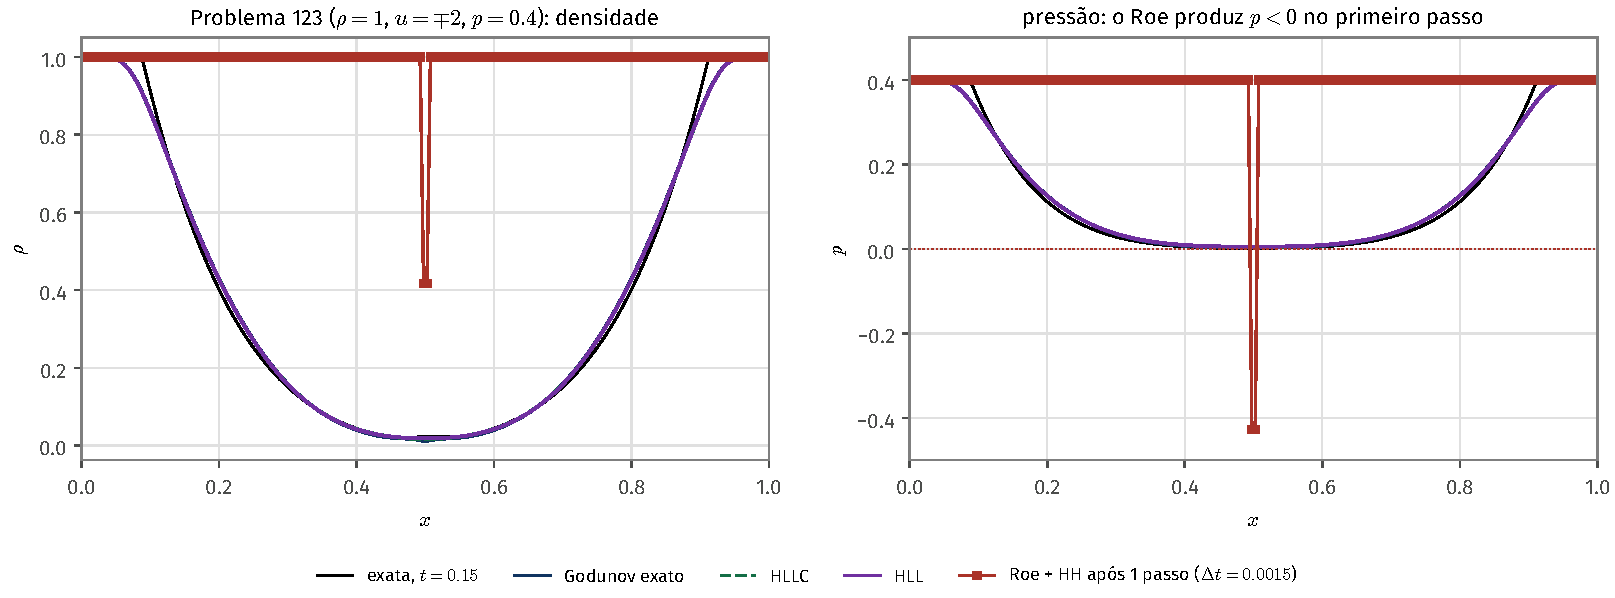
\includegraphics[width=\textwidth,height=0.4\textheight,keepaspectratio]{figs/roe_123.pdf}
\end{center}
\vspace{-0.1cm}
\begin{columns}[T]
\begin{column}{0.5\textwidth}
{\small \textbf{Problema 123} (Einfeldt et al., 1991): $\rho=1$ e $p=0.4$ dos dois lados, $u=-2$ à esquerda e $+2$ à direita. Duas rarefações fortes se afastam; no meio, $p^*=0.0019$ e $\rho^*=0.022$: quase vácuo, mas positivo.}
\end{column}
\begin{column}{0.5\textwidth}
{\small O Roe lineariza: $\hat u=0$, $\hat c^{\,2}=1.36$, e o estado estrela do problema \emph{linear} tem $\rho^*=1-2/\hat c<0$. No primeiro passo a célula vizinha fica com $p<0$. Baixar a CFL só adia; a correção de entropia não ajuda: o problema é a linearização.}
\end{column}
\end{columns}
\begin{mensagem}
Roe é o mais preciso dos aproximados e o menos robusto: pode sair do conjunto admissível. No bifásico com fase evanescente isso pesa mais que a nitidez do contato.
\end{mensagem}
\end{frame}

\begin{frame}{Outros fluxos, em uma linha cada, e a comparação em Sod}
\begin{itemize}
\item \textbf{Rusanov}: $Q=\max(|u|+c)$, a velocidade máxima; barato, positivo, borra tudo o que é lento.
\item \textbf{HLL} (Harten, Lax e van Leer, 1983): só duas ondas, $S_L<S_R$, e um estado entre elas fixado pela conservação, $\Fh=\dfrac{S_Rf_L-S_Lf_R+S_LS_R(u_R-u_L)}{S_R-S_L}$ para $S_L<0<S_R$; positivo com as velocidades de Einfeldt, mas borra o contato.
\item \textbf{HLLC} (Toro, Spruce e Speares, 1994): o HLL com a onda do contato de volta; nítido como o Roe, positivo como o HLL. É o fluxo do THM/MOOSE e do RELAP-7 (Encontros 3 e 4).
\end{itemize}
\begin{center}\scriptsize
\begin{tabular}{@{}l l l l l@{}}
\toprule
fluxo & dissipação $Q$ & ondas que resolve & entropia & positividade\\
\midrule
Rusanov & $\max_p|\lambda_p|$ & nenhuma & sim & sim\\
HLL / HLLC & $S_L$, $S_R$ (e $S_*$) & as extremas (e o contato) & sim & sim\\
Roe & $|\Ah|$ & todas, linearizadas & só com correção & \textbf{não}\\
Godunov exato & a física & todas & sim & sim\\
\bottomrule
\end{tabular}
\end{center}
\begin{mensagem}
Não existe ``o melhor fluxo'': existe o fluxo certo para o que se precisa garantir. Para o nosso problema, garantir é ficar no conjunto admissível.
\end{mensagem}
\end{frame}

\begin{frame}{Os fluxos no tubo de Sod: a diferença está no contato}
\begin{center}
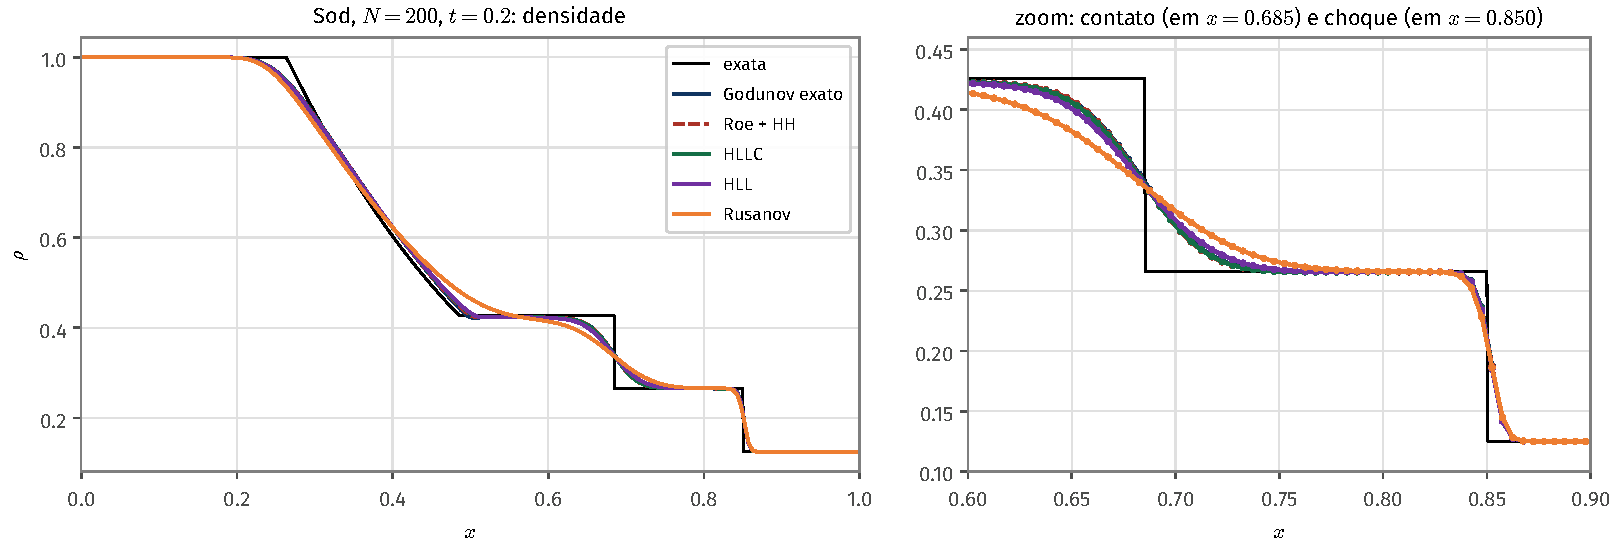
\includegraphics[width=\textwidth,height=0.64\textheight,keepaspectratio]{figs/sod_fluxos.pdf}
\end{center}
\vspace{-0.15cm}
{\footnotesize Sod, $N=200$, $t=0.2$, CFL $=0.8$. Godunov exato e Roe são indistinguíveis; HLLC fica entre eles e o HLL; Rusanov é o mais borrado. A diferença concentra-se no contato: para uma onda que viaja a $u^*=0.93$, Roe e HLLC dissipam com $|u^*|$, HLL e Rusanov com algo da ordem de $c$.}
\end{frame}


% =====================================================================
\section{Síntese}

\begin{frame}{Síntese em oito linhas}
\begin{columns}[T]
\begin{column}{0.5\textwidth}
\begin{enumerate}
\item Volumes finitos: a única incógnita é o fluxo na face. Esquema \emph{é} fluxo numérico.
\item Todo fluxo é média central menos $\tfrac12Q\,\Delta u$: $Q$ é a viscosidade do esquema; pouca oscila, muita borra.
\item Upwind: $Q=|a|$ e, em sistemas lineares, $Q=|A|$: cada onda dissipada com a sua $|\lambda_p|$. É Godunov para o caso linear.
\item Riemann: choque se $u_L>u_R$, leque se $u_L<u_R$; o valor na face é o ponto sônico quando o leque a contém. Em Euler, uma equação escalar $f(p^*)=0$.
\end{enumerate}
\end{column}
\begin{column}{0.5\textwidth}
\begin{enumerate}\setcounter{enumi}{4}
\item Godunov: reconstruir, evoluir exatamente, fazer a média; $\Fh=f(\RP(0))$. O erro está só na média.
\item Roe: a matriz constante que faz $(u_L,u_R)$ obedecer a Rankine--Hugoniot. Exato em saltos isolados; cego no ponto sônico (correção de entropia); pode perder a positividade.
\item HLL/HLLC: positivos e robustos; HLLC recupera o contato. Rusanov: o mais simples e o mais difusivo.
\item O fluxo fica. No Encontro 3 muda o que se entrega a ele: reconstrução limitada, rDG($P_0P_1$), positividade.
\end{enumerate}
\end{column}
\end{columns}
\end{frame}

\begin{frame}{Exercício para o próximo encontro (Python)}
\begin{exampleblock}{Problema A: Burgers, $\pd ut+\pd{}{x}\big(\tfrac{u^2}{2}\big)=0$ em $[-1,1]$, contornos transmissivos, $N=200$, CFL $=0.8$, até $t=0.5$}
Dados de Riemann com salto em $x=0$: (a) $u_L=1$, $u_R=-0.5$; (b) $u_L=-1$, $u_R=1$; (c) $u_L=-0.2$, $u_R=1$.
\end{exampleblock}
\vspace{-0.15cm}
\begin{enumerate}\footnotesize
\item Programe Godunov (fórmula do $\max/\min$), Roe sem correção e Roe com Harten--Hyman; plote os três com a solução exata em (a), (b) e (c). Em (c), descreva o que o Roe sem correção faz em $x=0$ e explique com $\hat a$ e $Q$.
\end{enumerate}
\vspace{-0.15cm}
\begin{exampleblock}{Problema B: Euler (gás ideal, $\gamma=1.4$) em $[0,1]$, contornos transmissivos, CFL $=0.8$}
Sod: $(\rho,u,p)=(1,0,1)$ para $x<0.5$ e $(0.125,0,0.1)$ para $x>0.5$, até $t=0.2$. Problema 123: $(1,-2,0.4)$ e $(1,2,0.4)$, até $t=0.15$.
\end{exampleblock}
\vspace{-0.15cm}
\begin{enumerate}\footnotesize\setcounter{enumi}{1}
\item Programe Roe com Harten--Hyman e Rusanov; use o solver exato fornecido (\texttt{riemann\_exato.py}) como referência. Em Sod, com $N=100,200,400$, plote $\rho$, $u$, $p$ e tabele $E_N=h\sum_j|\rho_j-\rho(x_j,0.2)|$ e $E_N/E_{2N}$ (esperado entre $\sqrt2$ e $2$). Verifique no código que $\sum_p\ah_p\rh_p=\Delta u$ e $\sum_p\lh_p\ah_p\rh_p=\Delta f$.
\item No problema 123, rode Rusanov e Roe: registre em que passo o Roe produz $p<0$ e confira à mão o valor $\rho^*=1-2/\hat c$ do slide.
\end{enumerate}
{\footnotesize Entrega antes do Encontro 3: script \texttt{.py}, figuras e uma página com a tabela e os comentários. Os scripts das figuras destes slides ficam disponíveis.}
\end{frame}

\begin{frame}{Referências}
\footnotesize
\begin{itemize}
\item S. K. Godunov. A difference method for numerical calculation of discontinuous solutions of the equations of hydrodynamics. \emph{Mat. Sb.} 47 (1959) 271--306.
\item P. L. Roe. Approximate Riemann solvers, parameter vectors, and difference schemes. \emph{J. Comput. Phys.} 43 (1981) 357--372.
\item A. Harten, J. M. Hyman. Self adjusting grid methods for one-dimensional hyperbolic conservation laws. \emph{J. Comput. Phys.} 50 (1983) 235--269.
\item A. Harten, P. D. Lax, B. van Leer. On upstream differencing and Godunov-type schemes for hyperbolic conservation laws. \emph{SIAM Rev.} 25 (1983) 35--61.
\item B. Einfeldt, C. D. Munz, P. L. Roe, B. Sjögreen. On Godunov-type methods near low densities. \emph{J. Comput. Phys.} 92 (1991) 273--295.
\item E. F. Toro, M. Spruce, W. Speares. Restoration of the contact surface in the HLL-Riemann solver. \emph{Shock Waves} 4 (1994) 25--34.
\item A. Harten, J. M. Hyman, P. D. Lax. On finite-difference approximations and entropy conditions for shocks. \emph{Comm. Pure Appl. Math.} 29 (1976) 297--322.
\item M. G. Crandall, A. Majda. Monotone difference approximations for scalar conservation laws. \emph{Math. Comp.} 34 (1980) 1--21.
\item P. Glaister. An approximate linearised Riemann solver for the Euler equations for real gases. \emph{J. Comput. Phys.} 74 (1988) 382--408.
\item R. J. LeVeque. \emph{Finite Volume Methods for Hyperbolic Problems}. Cambridge University Press, 2002.
\item E. F. Toro. \emph{Riemann Solvers and Numerical Methods for Fluid Dynamics}. 3.\textsuperscript{a} ed., Springer, 2009.
\end{itemize}
\end{frame}

\end{document}
